\chapter{Análisis y Diseño}

Las etapas iniciales de la metodología ``Cascada'' consisten en el análisis y diseño que son previos al inicio de la implementación del producto final. Es importante que estas fases sean completadas en su totalidad para que el desarrollo sea éxitoso. Este proyecto plantea un diseñado y desarrollo de 50 dias hábiles calendario con la distribución del tiempo definido según la complejidad de las tareas que implican cada una de las fases.\\

\section{Análisis}
Para el diseño de un sistema de video-vigilancia inteligente es necesario tener en cuenta los elementos principales que lo componen. Un sistema de video-vigilancia esta compuesto de cámaras individuales y un puesto central o servidor donde todas las conexiones convergen y se centralizan para su control. En el dispositivo central (servidor) se procesan las imágenes que las cámaras capturan y se convierten en video para ser visualizado en un monitor.\\

El sistema propuesto permite visualizar el video en vivo desde cualquier dispositivo con acceso a la red de internet además de que envía notificaciones automáticas en el instante en que se detecta: movimiento, fuego, humo o silueta de un intruso. El usuario recibe la notificación por correo electrónico el cual adjunta capturas y un enlace web para visualizar en vivo lo que esta captando la cámara.\\

% Los principales módulos del sistema son:
% \begin{itemize}
%     \item Módulo de cámara (Nodos)
%     \item Módulo de servidor (Analizador y noti)
%     % \item Servidor HTTP (Servicio que aplica el protocolo de la Web)
%     % \item Módulo SMTP (Módulo de envio de correo electrónico)
% \end{itemize}

En la figura \ref{fig:system_desing} se visualiza el esquema general del sistema propuesto. Las cámaras de video-vigilancia se encargan de capturar los fotogramas de video y se enlazan por medio de un socket o conector (uno por cada cámara) al servidor TCP. Cuando es registrada una nueva conexión, el sistema notifica al usuario por medio de un correo electrónico, compartiendo información relevante sobre la conexión de una nueva cámara. El servidor TCP que maneja todas las conexiones, realiza el análisis de los fotogramas de manera individual por cada cámara conectada por medio de una libreria de visión por computadora. Paralelamente se construye el video que se va a transmitir a partir de los fotogramas y es decodificado por medio de un conjunto de paquetes de software libre, los cuales arman las partes del archivo para el streaming de video por la red. Cuando un evento (fuego, humo, movimiento) es identificado, automáticamente se envia un correo electronico al usuario notificando una posible identificación de un evento.\\

\begin{figure}[H]
    \begin{center}
        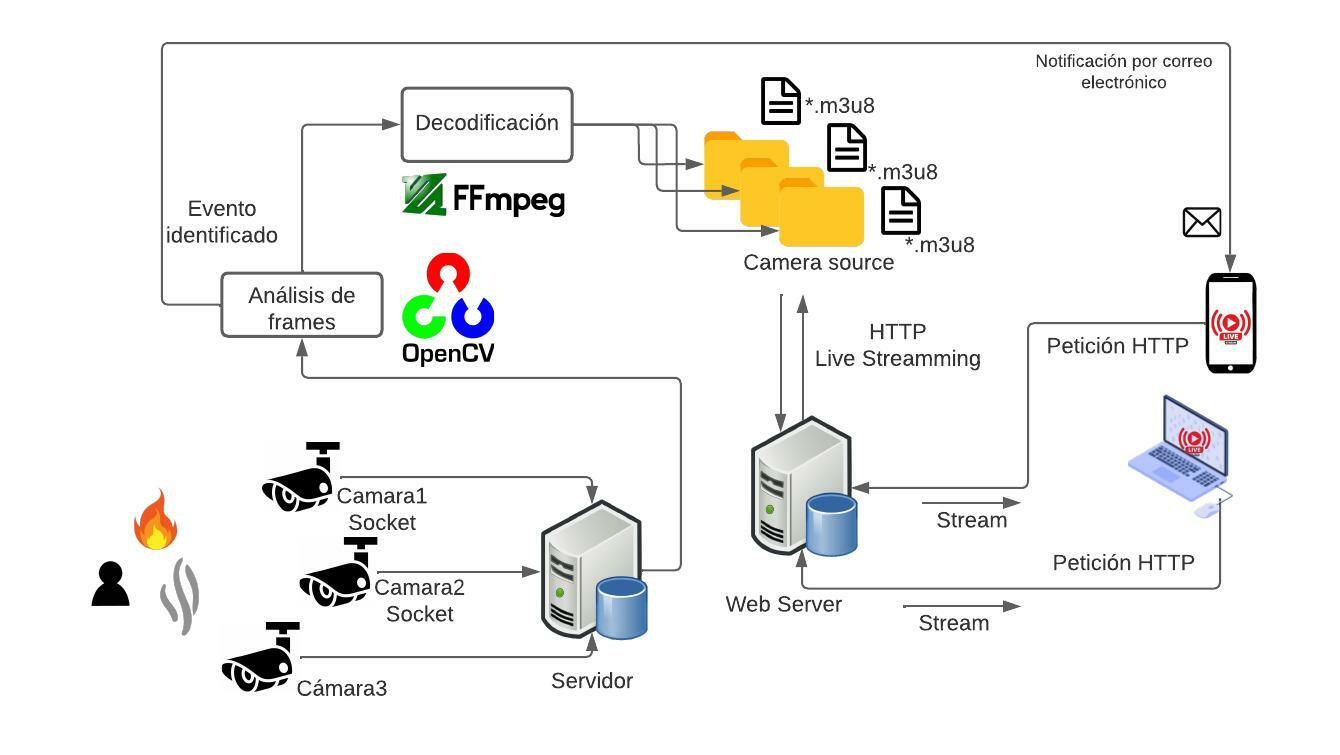
\includegraphics[width=17cm]{img/capitulo_4/main.jpeg}
        \caption{Diseño de interacción de los módulos del sistema de video-vigilancia.}
        Fuente : Elaboración propia
        \label{fig:system_desing}
    \end{center}
\end{figure}

\subsection{Definición de Requerimientos}
La definición de requerimientos es una de las actividades más importantes del desarrollo de software; de ello depende el resto de actividades del proyecto. Anteriormente se describe completamente el comportamiento del sistema que se desarrolla para la identificación de los requerimientos. Inicialmente se plantean los criterios de partida a tomar en cuenta en el diseño del sistema de video-vigilancia inteligente:

\begin{itemize}
    \item Costos altos en la infraestructura de transmisión de video en vivo.
    \item Las características de identificación automática, estan disponibles para sistemas de video-vigilancia de alto nivel.
    \item Una alerta inmediata puede minimizar el impacto de alguna situación que ponga en peligro la integridad de bienes materiales y humanos.
    \item Los usuarios finales son personas que a menudo dejan su hogar para salir a trabajar, y usan constamente su correo electrónico.
\end{itemize}

\subsubsection{Requerimientos Funcionales}
En esta fase es necesario delimitar el alcance y las capacidades del sistema planteado para la realización de la planificación inicial, estimación de tiempos, diseño y desarrollo. Para ello se define la lista de requerimientos funcionales del sistema de video-vigilancia inteligente.

\begin{table}[H]
    \caption{Lista de requerimientos funcionales }
    \label{tabla:req_funcionales}
    \begin{center}
        \begin{tabular}{ |c|l|} 
            \hline
            1. & Capturar fotogramas por medio de una o varias cámaras portatiles.\\ \hline
            2. & Visualizar fotogramas capturados en tiempo real (captura de video).\\  \hline
            3. & Notificar al usuario cuando una nueva cámara se conecta.\\  \hline
            4. & Enviar fotogramas capturados por medio de la red al servicio encargado de su análisis.\\ \hline
            5. & Análizar y procesar fotogramas capturados individualmente por cada cámara.\\  \hline
            6. & Permitir la recepción de fotogramas de varias fuentes hacia el servicio.\\ \hline
            7. & Transmitir los fotogramas convertidos en video en vivo desde fuentes diferentes.\\ \hline
            8. & Detectar movimiento a partir de los fotogramas recibidos desde distintas fuentes.\\ \hline
            9. & Detectar silueta humana a partir de los fotogramas recibidos desde distintas fuentes.\\ \hline
            10. & Detectar fuego y/o humo a partir de los fotogramas recibidos desde distintas fuentes.\\ \hline
            11. & Notificar al usuario por medio de un correo electrónico cuando se de una detección.\\ \hline
        \end{tabular}
    \end{center}
    \begin{center}
        Fuente: Elaboración propia.
    \end{center}
\end{table}

\subsubsection{Requerimientos No Funcionales}
Los requisitos no funcionales son aquellos relacionados con la calidad y el proceso de desarrollo del sistema. Los tipos de requisitos no funcionales son: rendimiento, disponibilidad, acecesibilidad, usabilidad, estabilidad, portabilidad, costo, operatividad, interoperabilidad, escalabilidad, concurrencia, mantenibilidad, interfaz, plazo de entrega y herramientas. Los requisitos no funcionales surgen de la necesidad del usuario, debido a las restricciones en el presupuesto y las herramientas utilizadas.\\

\begin{enumerate}
    \item  \textbf{Requisitos de interfaz} 
        \begin{itemize}
            \item Las cámaras tendran una interfaz que permita visualizar el trabajo que estan ejecutando.
            \item El servidor mostrará información necesaria sobre las tareas qeu realiza.
            \item El sistema deberá ser de fácil configuración.
            \item Las notificaciones por correo electrónico deberán ser visualmente agradables y estilizadas.
        \end{itemize}
    \item \textbf{Requisitos de portabilidad}
        \begin{itemize}
            \item Los módulos de cámara podran conectarse de forma cableada o inalámbrica.
        \end{itemize}
    \item \textbf{Requisitos de disponibilidad}
        \begin{itemize}
            \item La transmisión en vivo estará disponible cuando el usuario quiera visualizar lo que captan las cámaras.
        \end{itemize}
\end{enumerate}

\section{Planificación}
Todas las fases del modelo cascada son planificadas según la complejidad y tareas que presenta cada fase. Dado que cada fase debe culminarse por completo para pasar a la siguiente o en su defecto requerir mínimas modificaciones para regresar a la fase anterior, se plantea una planificación de 60 días hábiles que se visualiza en la tabla \ref{tabla:planning}.\\

\begin{table}[H]
    \caption{Tabla de planificación según fases del modelo Cascada.}
    \label{tabla:planning}
    \begin{center}
        \begin{tabular}{|c|l|c|c|c|}
            \hline
            \textbf{Num.} & \textbf{Fase del modelo Cascada}  &  \textbf{Fecha inicial} & \textbf{Fecha final} & \textbf{Duración (días)}\\ \hline
            \textbf{1.} & Fase de análisis        & 6-jun        & 17-jun        & 10        \\ \hline
            \textbf{2.} & Fase de diseño del sistema       & 20-jun        & 8-jul        & 15        \\ \hline
            \textbf{3.} & Fase de implementación        & 11-jul        & 19-ago        & 30        \\ \hline
            \textbf{4.} & Fase de pruebas        & 22-ago         &   2-sep     &    10     \\ \hline
            \textbf{5.} & Fase de mantenimiento        & 5-sep        & 9-sep        & 5        \\ \hline
        \end{tabular}
        \begin{center}            
            Fuente: Elaboración propia.
        \end{center}
    \end{center}
\end{table}

En la figura \ref{fig:gannt} se visualiza e diagrama de Gannt en base a la planificación expresada en la anterior tabla.
\begin{figure}[H]
    \begin{center}
        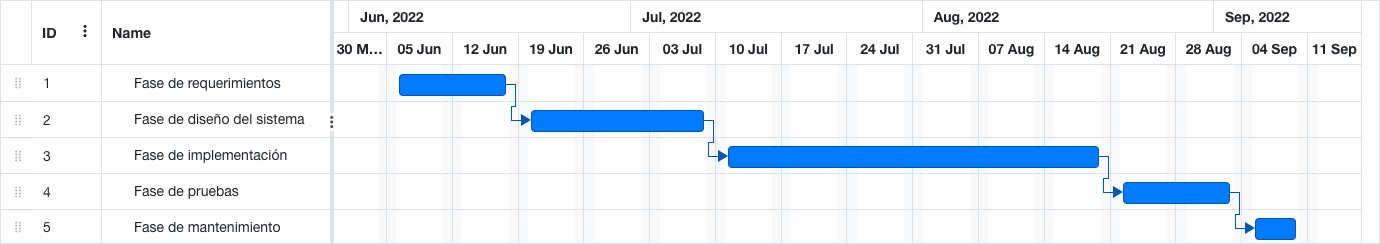
\includegraphics[width=18cm]{img/capitulo_4/gant.png}
    \end{center}
    \begin{center}
        \caption{Diagrama de Gannt.}
        Fuente : Elaboración propia
        \label{fig:gannt}
    \end{center}
\end{figure}

\section{Diseño}
El diseño del sistema de video-vigilancia se divide y se desarrolla según los módulos que componen el sistema completo:
\begin{itemize}
    \item Módulo de cámaras
    \item Módulo de servidor
\end{itemize}

\subsection{Módulo de cámaras}
Este módulo es el encargado de controlar y conectar la cámara al servidor TCP. Esta planificado para funcionar en un dispositivo portatil como ser una raspberry. Gracias a la
\subsubsection{Diseño de interfaz}
Este es un esbozo de lo que será implementado como la interfaz del módulo de cámara que permite la visualizacion de fotogramas capturados, configuración de la conexión y verificar el estado del envio de los fotogramas al servidor.
\subsubsection{Diagrama de secuencia}
Este diagrama consiste en describir el proceso de conexión entre la cámara y el servidor hasta que se empieza el envio de los fotogramas.

En la figura \ref{fig:diagrama_interaccion_general}.
\begin{figure}[H]
    \begin{center}
        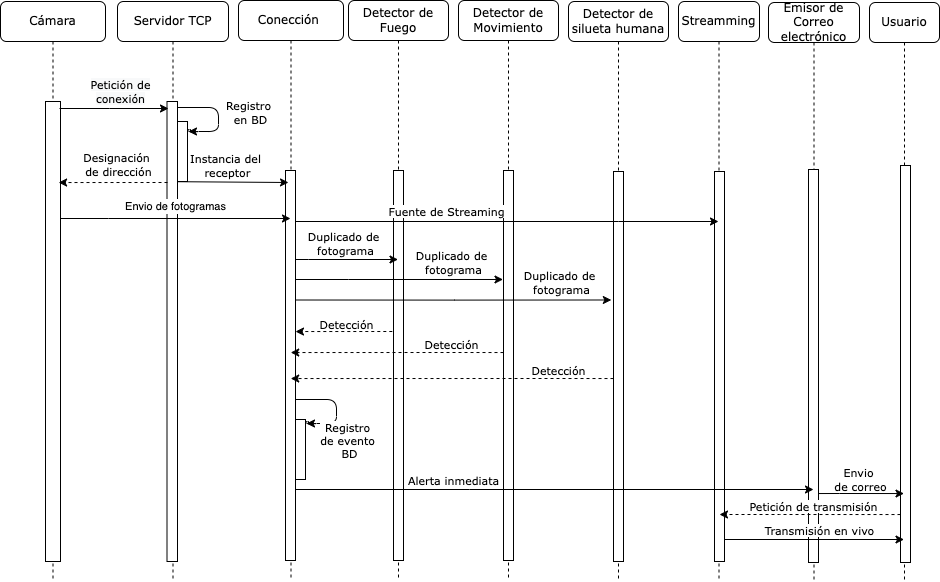
\includegraphics[width=17cm]{img/capitulo_4/interaccion.png}
    \end{center}
    \begin{center}
        \caption{Diagrama de interacción entre los módulos del sistema.}
        Fuente: Elaboración propia.
        \label{fig:diagrama_interaccion_general}
    \end{center}
\end{figure}

\subsubsection{Diagrama de estado}
Se estudia los casos en los que el usuario interactura con el módulo de cámara.
\begin{itemize}
    \item Usuario inicializa la cámara
    \item Ingresa la configuracion
    \item Si hay un dispositivo con la misma configuracion se recahza la conexión.
    \item sigue el proceso exitoso.
\end{itemize}
\subsubsection{Diagrama de clases}

En la figura \ref{fig:camera_clases} se describe el modelo de clases y a continuacion se detalla los métodos de las clases.\\
\begin{figure}[H]
    \begin{center}
        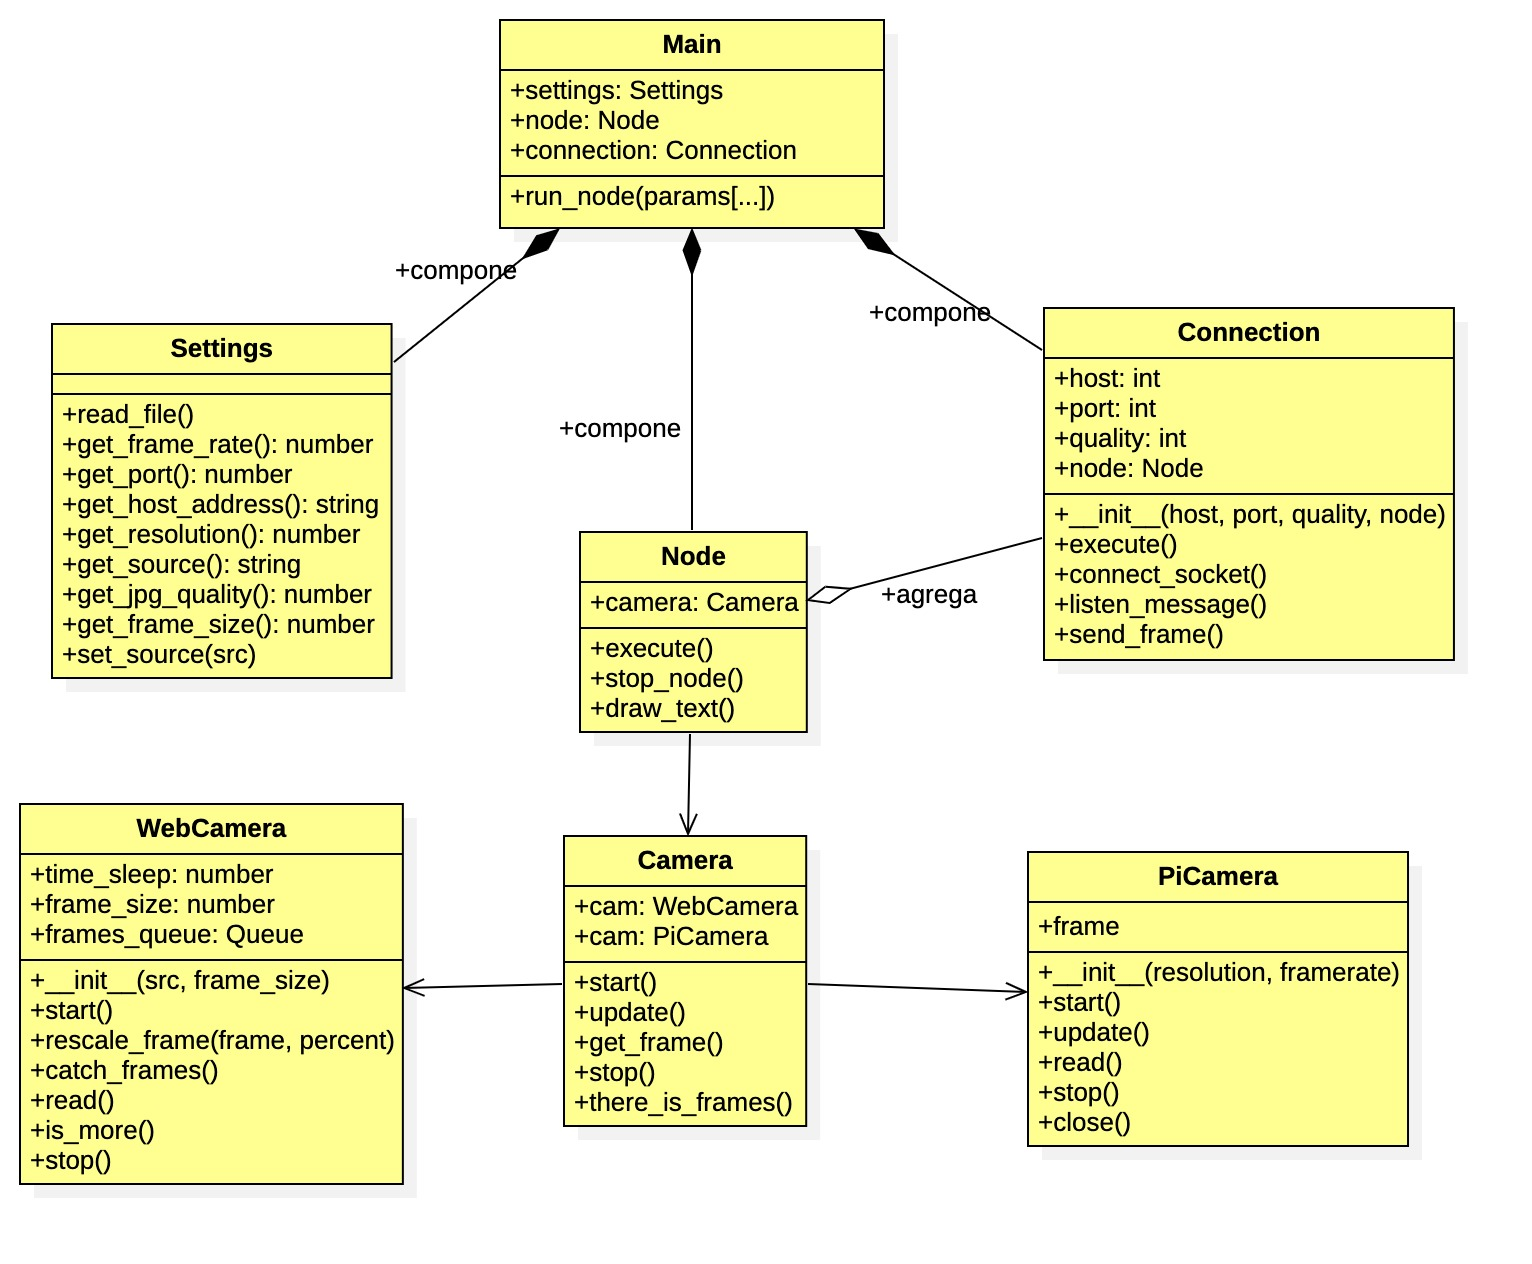
\includegraphics[width=15cm]{img/capitulo_4/camera_clases.jpg}
        \caption{Diagrama de clases del módulo de cámara.}
        Fuente : Elaboración propia
        \label{fig:camera_clases}
    \end{center}
\end{figure}

\subsection{Módulo de servidor}
El servidor que se encarga de la transmision
\subsubsection{Diagrama de secuencia}
Se describe el proceso entre el servidor y la cámara para el respectivo análisis de los frames
\subsubsection{Diagrama de estado}
Describe el funcionamiento como se manejan las conexiones internas.

\subsubsection{Diagrama de clases}
Se visualiza el diagrama de clases del servidor.
\subsubsection{Diagrama de la base de datos}
En la figura \ref{fig:db_diagram} se visualiza el diseño de entidades de la base de datos\\.
\begin{figure}[H]
    \begin{center}
        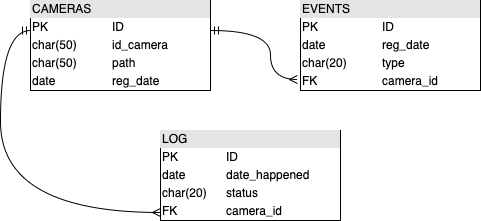
\includegraphics[width=10cm]{img/capitulo_4/db.png}
        % \caption{Diagrama de clases del módulo de cámara}
    \end{center}
    \begin{center}
        \caption{Diagrama entidad-relación.}
        Fuente : Elaboración propia
        \label{fig:db_diagram}
    \end{center}
\end{figure}

\subsubsection{Diseño de notificación por correo electrónico}
Esbozo del contenido del correo electrónico.